%%% LaTeX Template: Two column article
%%%
%%% Source: http://www.howtotex.com/
%%% Feel free to distribute this template, but please keep to referal to http://www.howtotex.com/ here.
%%% Date: February 2011

%%% Preamble
\documentclass[	DIV=calc,%
							paper=a4,%
							fontsize=12pt,%
							onecolumn]{scrartcl}	 					% KOMA-article class

\usepackage{lipsum}													% Package to create dummy text
\usepackage[brazil]{babel}										% English language/hyphenation
\usepackage[protrusion=true,expansion=true]{microtype}				% Better typography
\usepackage{amsmath,amsfonts,amsthm}					% Math packages
\usepackage[pdftex]{graphicx}									% Enable pdflatex
\usepackage[svgnames]{xcolor}									% Enabling colors by their 'svgnames'
\usepackage[hang, small,labelfont=bf,up,textfont=it,up]{caption}	% Custom captions under/above floats
\usepackage{epstopdf}												% Converts .eps to .pdf
\usepackage{subfig}													% Subfigures
\usepackage{booktabs}												% Nicer tables
\usepackage{fix-cm}													% Custom fontsizes
\usepackage[utf8]{inputenc}
\usepackage[top=2.5cm, bottom=2.5cm, left=2.5cm, right=2.5cm]{geometry}
\usepackage[ddmmyyyy]{datetime}
\addto\captionsenglish{%
	\renewcommand\tablename{Tabela}
	\renewcommand\figurename{Figura}
} 
 

 
%%% Custom sectioning (sectsty package)
\usepackage{sectsty}													% Custom sectioning (see below)
\allsectionsfont{%															% Change font of al section commands
	\usefont{OT1}{phv}{b}{n}%										% bch-b-n: CharterBT-Bold font
	}

\sectionfont{%																% Change font of \section command
	\usefont{OT1}{phv}{b}{n}%										% bch-b-n: CharterBT-Bold font
	}



%%% Headers and footers
\usepackage{fancyhdr}												% Needed to define custom headers/footers
	\pagestyle{fancy}														% Enabling the custom headers/footers
\usepackage{lastpage}	

% Header (empty)
\lhead{}
\chead{}
\rhead{}
% Footer (you may change this to your own needs)

%% ====================================
%% ====================================
%% mude o rodape  do projeto
%% ====================================
%% ====================================

\lfoot{\footnotesize \texttt{Template relatório} \textbullet ~Processo desenvolvimento do FastProject}


\cfoot{}
\rfoot{\footnotesize página \thepage\ de \pageref{LastPage}}	% "Page 1 of 2"
\renewcommand{\headrulewidth}{0.0pt}
\renewcommand{\footrulewidth}{0.4pt}



%%% Creating an initial of the very first character of the content
\usepackage{lettrine}
\newcommand{\initial}[1]{%
     \lettrine[lines=3,lhang=0.3,nindent=0em]{
     				\color{DarkGoldenrod}
     				{\textsf{#1}}}{}}



%%% Title, author and date metadata
\usepackage{titling}															% For custom titles

\newcommand{\HorRule}{\color{DarkGoldenrod}%			% Creating a horizontal rule
									  	\rule{\linewidth}{1pt}%
										}

\pretitle{\vspace{-30pt} \begin{flushleft} \HorRule 
				\fontsize{50}{50} \usefont{OT1}{phv}{b}{n} \color{DarkRed} \selectfont 
				}

%% ====================================
%% ====================================
%% mude o titulo  do projeto
%% ====================================
%% ====================================

\title{Processo de desenvolvimento de sistema para gerenciamento de projetos}					% Title of your article goes here

%% ====================================



\posttitle{\par\end{flushleft}\vskip 0.5em}

\preauthor{\begin{flushleft}
					\large \lineskip 0.5em \usefont{OT1}{phv}{b}{sl} \color{DarkRed}}
\author{Pablo Lima Flores }  	% Author name goes here


\postauthor{\footnotesize \usefont{OT1}{phv}{m}{sl} \color{Black} 
					\\Universidade Tecnológica Federal do Paraná - Câmpus Cornélio Procópio 								% Institution of author
					\par\end{flushleft}\HorRule}

\date{}																				% No date




%%% Begin document
\begin{document}
\maketitle
\thispagestyle{fancy} 	
\thispagestyle{empty}		% Enabling the custom headers/footers for the first page 
% The first character should be within \initial{}




%% ====================================
%% ====================================
%% mude o resumo  do projeto
%% ====================================
%% ====================================
\initial{V}\textbf{isando maior liberdade para elaboração do relatório, será utilizado uma equipe de 7 pessoas de uma empresa fictícia cujo objetivo é o desenvolvimento de um sistema web para cadastro e gerenciamento de projetos. 
	Esta demanda veio de um Escritório de Gerenciamento de Projeto da empresa ProjectX, cliente cujos usuários finais possuem com conhecimento especializado na área.}

%% ====================================
\begin{figure}
	\centering
	
\includegraphics{utfpr}
\end{figure}

\vspace{3cm}
\centerline{\textit{\textbf{\today}}}

\clearpage
    \renewcommand*\listfigurename{Lista de figuras}
\listoffigures

\clearpage
\renewcommand{\contentsname}{Sumário}
\tableofcontents
\clearpage

%% ====================================
%% ====================================
%% Inicio do texto
%% ====================================
%% ====================================
\section{Introdução}

\begin{itemize}
\item Neste documento será abordado uma visão geral do processo de desenvolvimento do FastProject um software para utilização web, que visa o registro e gerenciamento de projetos a partir da inserção de um pré-projeto, que passará por um processo de aprovação por um usuário com permissão correspondente, para então pode ser inicializado. 
\item Primeiramente será desenvolvida uma versão web responsível.
\item Futuramente, pretende-se desenvolver versões mobile Android e IOs.
\item A elaboração deste documento está sendo desenvolvida por Pablo Lima Flores.
\end{itemize}

\section{Processo}
Nesta seção será apresentado um diagrama que representa o processo geral de desenvolvimento do sistema.

\subsection{Papeis}
A equipe designada para o desenvolvimento e execução do processo é formada por 7 integrantes, e é composta por:
\begin{itemize}
\item 1 Gerente de Projeto;
\item 1 Analista de Requisitos;
\item 1 Representante do cliente;
\item 3 Programadores;
\item 1 Analista de Testes.
\end{itemize}

\subsection{Atividades}
O Gerente de Projeto é o responsável por liderar a equipe e acompanhar todas as etapas do mesmo, desde o contato inicial com o cliente até a ultima entrega. A partir deste acompanhamento ele pode ir direcionando a equipe e tomando as decisões de acordo com o cenário apresentado.
\\O Analista de Requisitos é responsável por efetuar o gerenciamento dos requisitos do cliente, desde o levantamento inicial, passando pela documentação de especificação de requisitos para repassar a equipe de desenvolvimento para implementação.
\\O Representante do Cliente será o contato principal para todos os outros da equipe no que tange repassar as informações complementares dos processos relacionados ao produto esperado e acompanha o andamento do projeto para ser o intermediário entre o cliente e a equipe do projeto.
\\Para o desenvolvimento deste projeto serão necessários 3 programadores fullstack, especializados em desenvolvimento de sistemas web em Java com front-end em Angular 7.
\\Para melhor eficiência no desenvolvimento e visando aumentar a confiabilidade no produto, foi designado um Analista de Testes para validação dos itens desenvolvidos nas sprints.
\\A figura \ref{fig1} representa o processo geral.

\begin{figure}
	\centering
	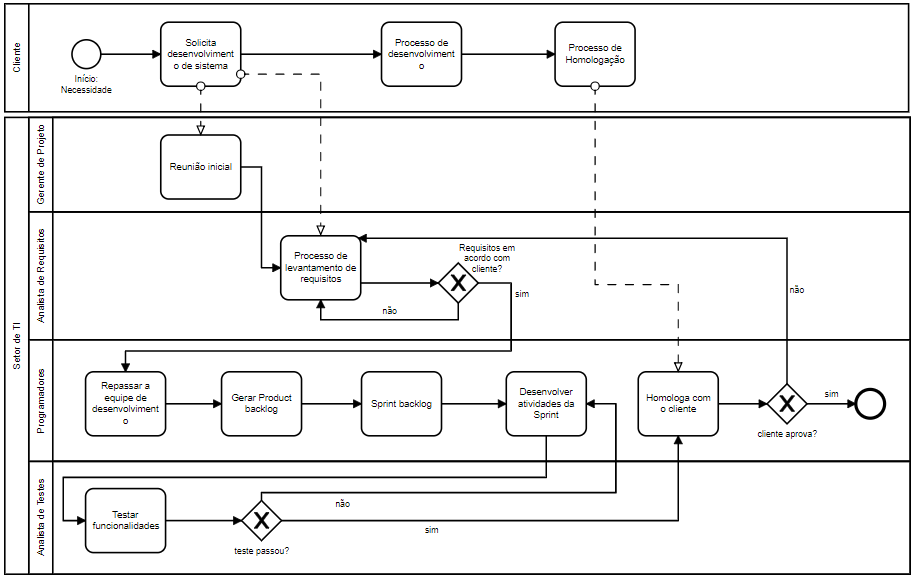
\includegraphics[width=\textwidth]{fig1}
	\caption{Processo de desenvolvimento}
	\label{fig1}
\end{figure}

\section{Execução do projeto}

Para a execução deste projeto foi definido a utilização de métodos ágeis para o desenvolvimento, mais especificadamente o Scrum.

\subsection{Backlog e sprints}
Como backlog do projeto pode-se definir as seguintes atividades:
\begin{itemize}
	\item Reunião com equipe para início do processo de análise e desenvolvimento do FastProject; (Gerente de Projeto)
	\item Gerar Documentação de levantamento e especificação de requisitos; (Analista de Requisitos)
	\item Modelar inicial diagrama de classes de acordo com as funcionalidades definidas nos requisitos; (Analista de Requisitos)
	\item Criar projeto (software) no GIT e efetuar configurações básicas; (Gerente de Projeto)
	\item Definição do layout e identificação visual do sistema; (Gerente do Projeto)
	\item Desenvolver CRUD de usuário, perfis de acesso e funcionalidade de controle de acesso ao sistema (login); (Programador)
	\item Teste CRUD de usuário, perfis de acesso e funcionalidade de controle de acesso ao sistema; (Analista de Testes)
	\item Desenvolvimento dos CRUDs básicos (sessão administrativa); (Programador)
	\item Teste dos CRUDs básicos (sessão administrativa); (Analista de Testes)
	\item Desenvolvimento da funcionalidade de cadastro do pré-projeto; (Programador)
	\item Testes da funcionalidade de cadastro do pré-projeto; (Analista de Teste)
	\item Adicionar processo de aprovação do pré-projeto, de acordo com o perfil do usuário; (Programador)
	\item Testes processo de aprovação do pré-projeto, de acordo com o perfil do usuário; (Analista de Testes)
	\item Desenvolvimento das funcionalidades referentes ao termo de Abertura do Projeto(TAP); (Programador)
	\item Testes das funcionalidades referentes ao termo de Abertura do Projeto(TAP); (Analistas de Testes)
	\item Desenvolvimento do cadastro da Matriz de Interessados; (Programador)
	\item Testes no cadastro da Matriz de Interessados; (Analista de Testes)
	\item Desenvolvimento do cadastro dos Recursos Humanos e Equipamentos; (Programador)
	\item Testes no cadastro dos Recursos Humanos e Equipamentos; (Analista de Testes)
	\item Desenvolvimento do cadastro da Matriz de Responsabilidades; (Programador)
	\item Testes no cadastro da Matriz de Responsabilidades; (Analista de Teste)
	\item Desenvolvimento da funcionalidade de gestão do cronograma do projeto; (Programador)
	\item Testes na funcionalidade de gestão do cronograma do projeto; (Analista de Testes)
	\item Desenvolvimento do cadastro da Matriz de Risco; (Programador)
	\item Desenvolvimento do cadastro da Matriz de Risco; (Analista de Testes)
	\item Desenvolvimento das rotinas referentes a execução do projeto e monitoramento; (Programador)
	\item Teste das rotinas referentes a execução do projeto e monitoramento; (Analista de Testes)
	\item Desenvolver cadastro e geração de relatório do termo de encerramento; (Programador)
	\item Teste cadastro e geração de relatório do termo de encerramento; (Analista de Testes)
	\item Criar relatórios; (Programador)
	\item Testes relatórios; (Analista de Testes)
\end{itemize}

As sprints terão duração média de 2 semanas, podendo ser o período alterado de acordo com a complexidade das funcionalidades ou fatores externos.
 


\subsection{Estado atual}
O estado atual dos processo envolvendo gerenciamento de projetos na ProjecX é efetuado de forma "semi-manual". Tendo os pré-projetos definidos e organizados manualmente em um canvas em um mural na parede na sala de reuniões. A partir do momento em que o projeto é aprovado para ser executado, todas as informações são gerenciadas em planilhas complexas, de difícil manutenção.
Com o a entrega do novo software, pretende-se terminar com estas dificuldades e agilizar o processos de gerenciamento dos projetos.


\end{document}